\documentclass[UTF8]{ctexart}
\usepackage{lmodern}
\usepackage{amsmath}
\usepackage{graphicx}
\usepackage{float}%提供float浮动环境
\usepackage{booktabs}%提供命令\toprule、\midrule、\bottomrule
\usepackage{geometry}

\geometry{a4paper,left=2cm,right=2cm,top=2cm,bottom=2cm}

\title{{电子技术基础实验} \\ \textbf{实验二\ 三极管放大电路}}
\author{\\\textbf{祝尔乐}
        \\\textbf{未央-电01}
        }
\date{\textbf{\today}}

\begin{document}
\maketitle

\section*{一.实验目的}
1、掌握三极管放大电路静态工作点的测量方法。

2、掌握放大电路主要性能参数的测量方法。

3、熟悉用 LTspice 仿真电路。

\section*{二.实验内容}

\subsection*{1.测量三极管2N3904的输入输出特性}
\begin{figure}[htbp]
   \centering
   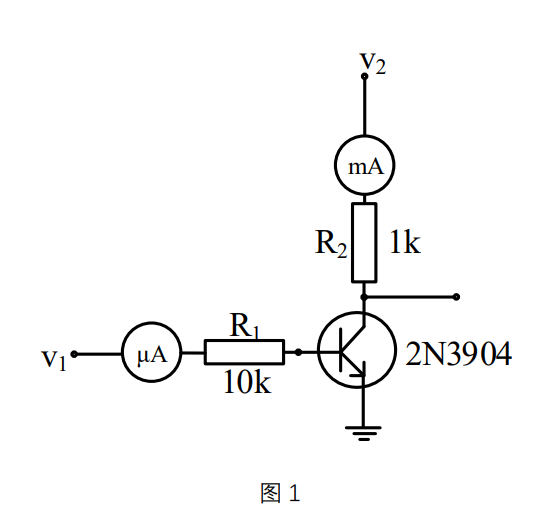
\includegraphics[width=0.40\textwidth]{1-电路图.png}
\end{figure}

采用图1的电路测量三极管2N3904的输入输出特性。通过调整V1,V2的值,
使三极管的$U_{BE}$和$U_{CE}$不断发生变化,测量$U_{BE}$, $U_{CE}$,$I_C$,$I_B$
的值就可以得到三极管的输入输出特性。

输入特性测量结果见下表:

\begin{table}[H]
        \centering
        \caption{\label{表1}\textbf{三极管的输入特性测量}}
        \begin{tabular}{cccccccccc}
        \toprule
        $U_{CE} = 0.0V$ & $U_{BE}/V$      & 0.504 & 0.537 & 0.555 & 0.572 & 0.574 & 0.578 & 0.590 & 0.597 \\
                        & $I_{B}/\mu A$   & 0.8   & 5.2   & 9.0   & 15.0  & 18.0  & 21.0  & 32.0  & 42.0 \\
        \midrule
        $U_{CE} = 2.0V$ &$U_{BE}/V$      & 0.635 & 0.648 & 0.658 & 0.667 & 0.678 & 0.680 & 0.681 & 0.682  \\
                        &$I_{B}/\mu A$   & 0.8   & 4.8   & 9.2   & 15.8  & 26.0  & 34.2  & 43.8  & 46.5   \\
        \bottomrule
        \end{tabular}
\end{table}

画出输入特性的图:
\begin{figure}[htbp]
        \centering
        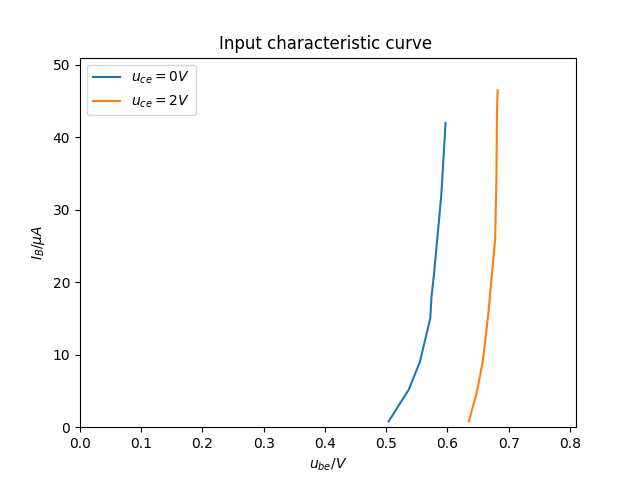
\includegraphics[width=0.55\textwidth]{输入特性曲线.png}
    \end{figure}

输出特性曲线见下表:

\begin{table}[H]
        \centering
        \caption{\label{表2}\textbf{三极管的输出特性测量}}
        \begin{tabular}{cccccccccc}
        \toprule
        $I_B=34\mu A$ & $U_{CE}/V$ & 0.808 & 2.13 & 2.84 & 3.72 & 5.12 & 6.03 & 7.12 & 8.32 \\
                      & $I_C/mA$   & 0.8   & 2.4 & 3.3 & 4.2 & 5.6 & 6.0 & 6.2 & 6.2 \\
        \midrule
        $I_B = 22\mu A$ & $U_{CE}/V$ & 1.09 & 1.90 & 2.76 & 3.50 & 4.37 & 5.80 & 7.20 & 8.24\\
                        & $I_C/mA$   & 1.0 & 2.0 & 3.0 & 4.0 & 4.0 & 4.0 & 4.0 & 4.0\\
        \midrule
        $I_B = 10\mu A$ & $U_{CE}/V$ & 0.69 & 1.49 & 2.36 & 3.26 & 4.40 & 5.56 & 7.20 & 8.12 \\
                        & $I_C/mA$   &  0.8 & 1.6 & 2.0 & 2.1 & 2.1 & 2.0 &2.0 & 2.0     \\        
        \bottomrule
        \end{tabular}
\end{table}

可以估算出该三极管的$\beta$的值约为200。

画出输出特性的图:
\begin{figure}[htbp]
    \centering
    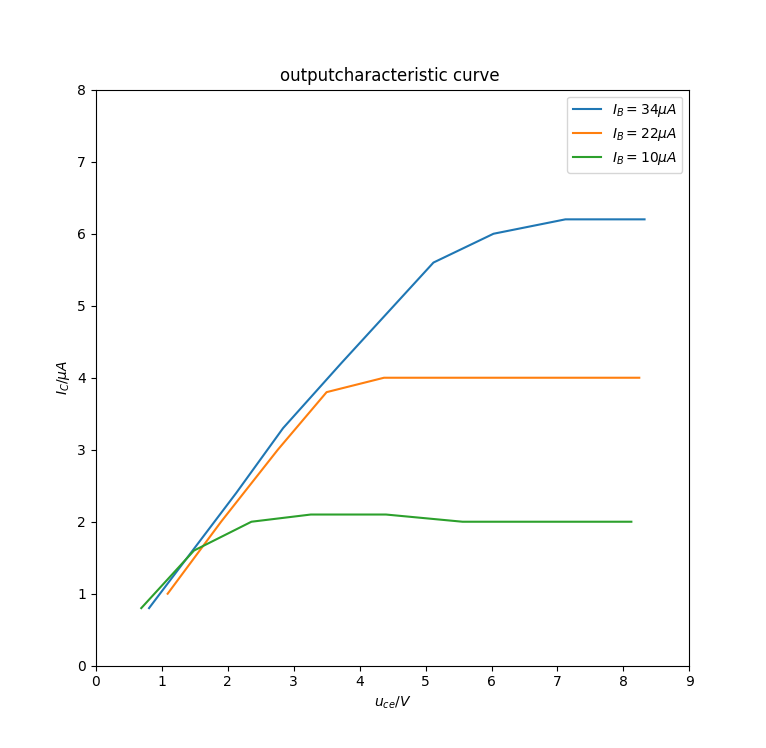
\includegraphics[width=0.55\textwidth]{输出特性曲线.png}
\end{figure}

\subsection*{2.共射级放大电路分析}
搭建图 2 所示电路。$VCC = 15V, R_L = 10k \Omega$。

\begin{figure}[htbp]
    \centering
    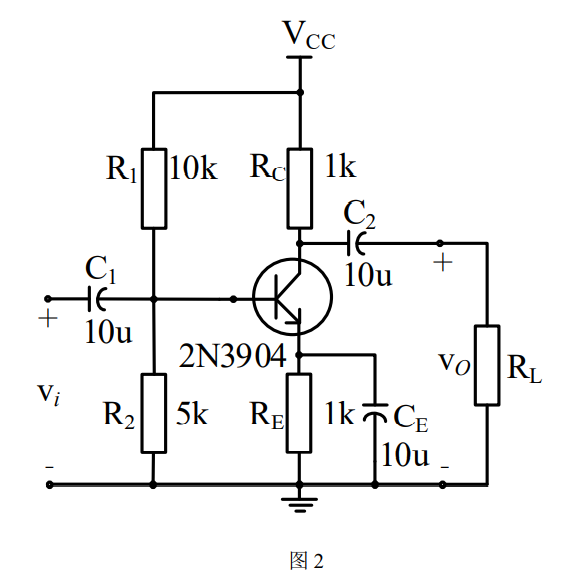
\includegraphics[width=0.40\textwidth]{2-电路图.png}
\end{figure}

\subsubsection*{(1)测量电路的静态工作点}

测量结果如下表:

\begin{table}[H]
    \centering
    \caption{\label{表3}\textbf{静态工作点测量}}
    \begin{tabular}{ccc}
    \toprule
            $U_E/V$ & $U_B/V$ &  $U_C/V$\\
    \midrule
            4.258 & 4.91 & 10.36\\            
    \bottomrule
    \end{tabular}
\end{table}

\subsubsection*{(2)测量电压放大倍数 、输入电阻$R_i$、输出电阻$R_o$;设置正弦波输入信号,
有效值 $VRMS \approx 5mV$,频率为 10kHz}

得到的波形为:
\begin{figure}[htbp]
    \centering
    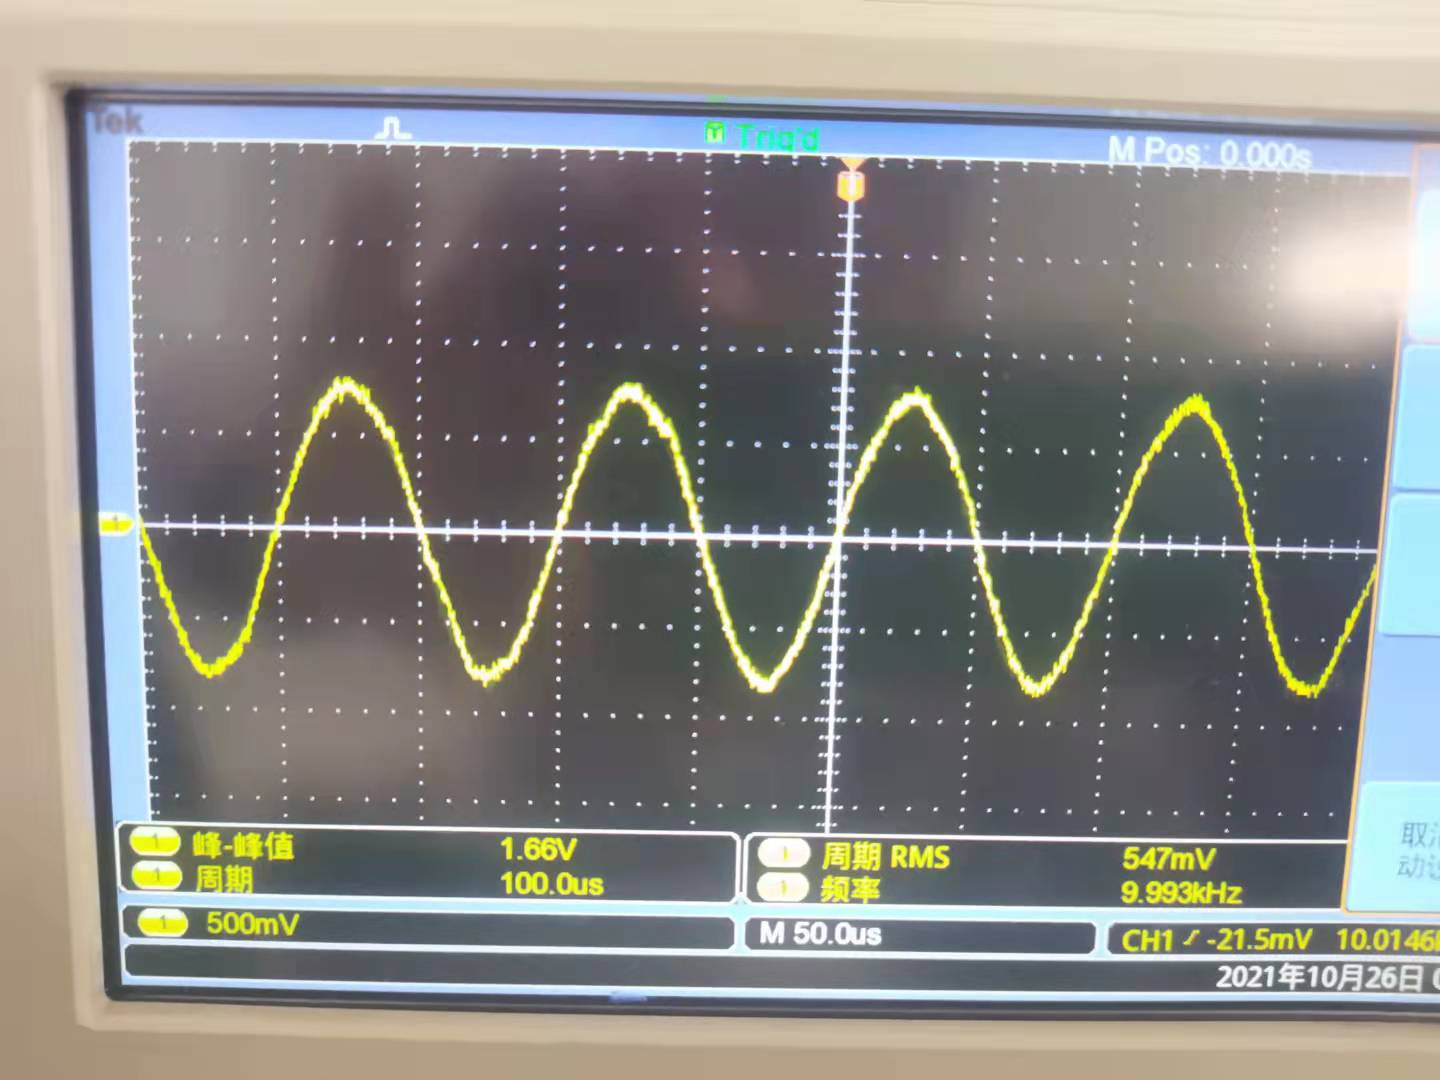
\includegraphics[width=0.60\textwidth]{2-2.jpg}
\end{figure}

电压放大倍数为:
\begin{align}
        A_u = \frac{U_o}{U_i} = \frac{1.66}{10\sqrt{2}m} \approx 117.4  
\end{align}


采用附件中的方法测量输入电阻,$R_1 = 10K\Omega,U_S = 50mVrms$,
使得$U_i' = 56.6mV, U_i = 9.62mV$,

\begin{align}
        R_i = \frac{U_i}{U_i' - U_i}R_1 \approx 2k \Omega
\end{align}

采用附件中的方法测量输出电阻,
$U_S = 10mVrms, R_L=10k\Omega $,
测出$U_o' =1.2mv ,U_{OL} = 1.1mv$,

\begin{align}
        R_o = (\frac{U_o'}{U_{oL}} - 1)R_L \approx 1k\Omega
\end{align}

\subsubsection*{(3)改变输入信号频率(100Hz、1kHz……),测量输出信号幅值,画出幅
频特性曲线}

改变输入信号频率,测量输出信号的幅值,测量结果如下表:

\begin{table}[H]
        \centering
        \caption{\label{表4}\textbf{静态工作点测量}}
        \begin{tabular}{ccc}
        \toprule
                $f/Hz$ & $U_O/V(峰-峰值)$ & $A_u$\\
        \midrule
                10 & 0.0328 & 2.32\\ 
                100 & 0.22 & 15.56\\
                500 & 0.43 & 30.46\\
                1k & 0.78 & 55.15\\
                5k & 1.48 & 104.56\\
                10k & 1.62 & 114.55\\
                100k & 1.72 & 121.62\\
        \bottomrule
        \end{tabular}
\end{table}

\begin{figure}[htbp]
        \centering
        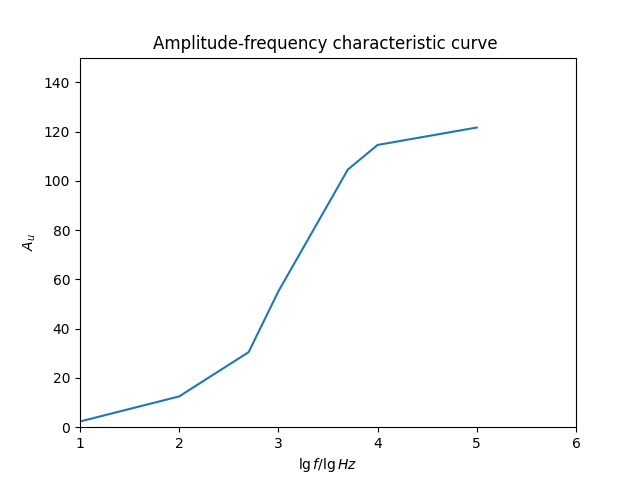
\includegraphics[width=0.40\textwidth]{幅频特性曲线.png}
\end{figure}

\subsubsection*{(4)在发射极与$R_E$之间串联一个100Ω电阻(保持$C_E$与 $R_E$ 并联),测量输
出波形及电压放大倍数,与上面结果比较,分析发射极电阻对放大电路的影响}

串联$100\Omega$电阻,输入电压仍采用$5mVrms, 10kHz$,得到输出电压的波形

\begin{figure}[htbp]
        \centering
        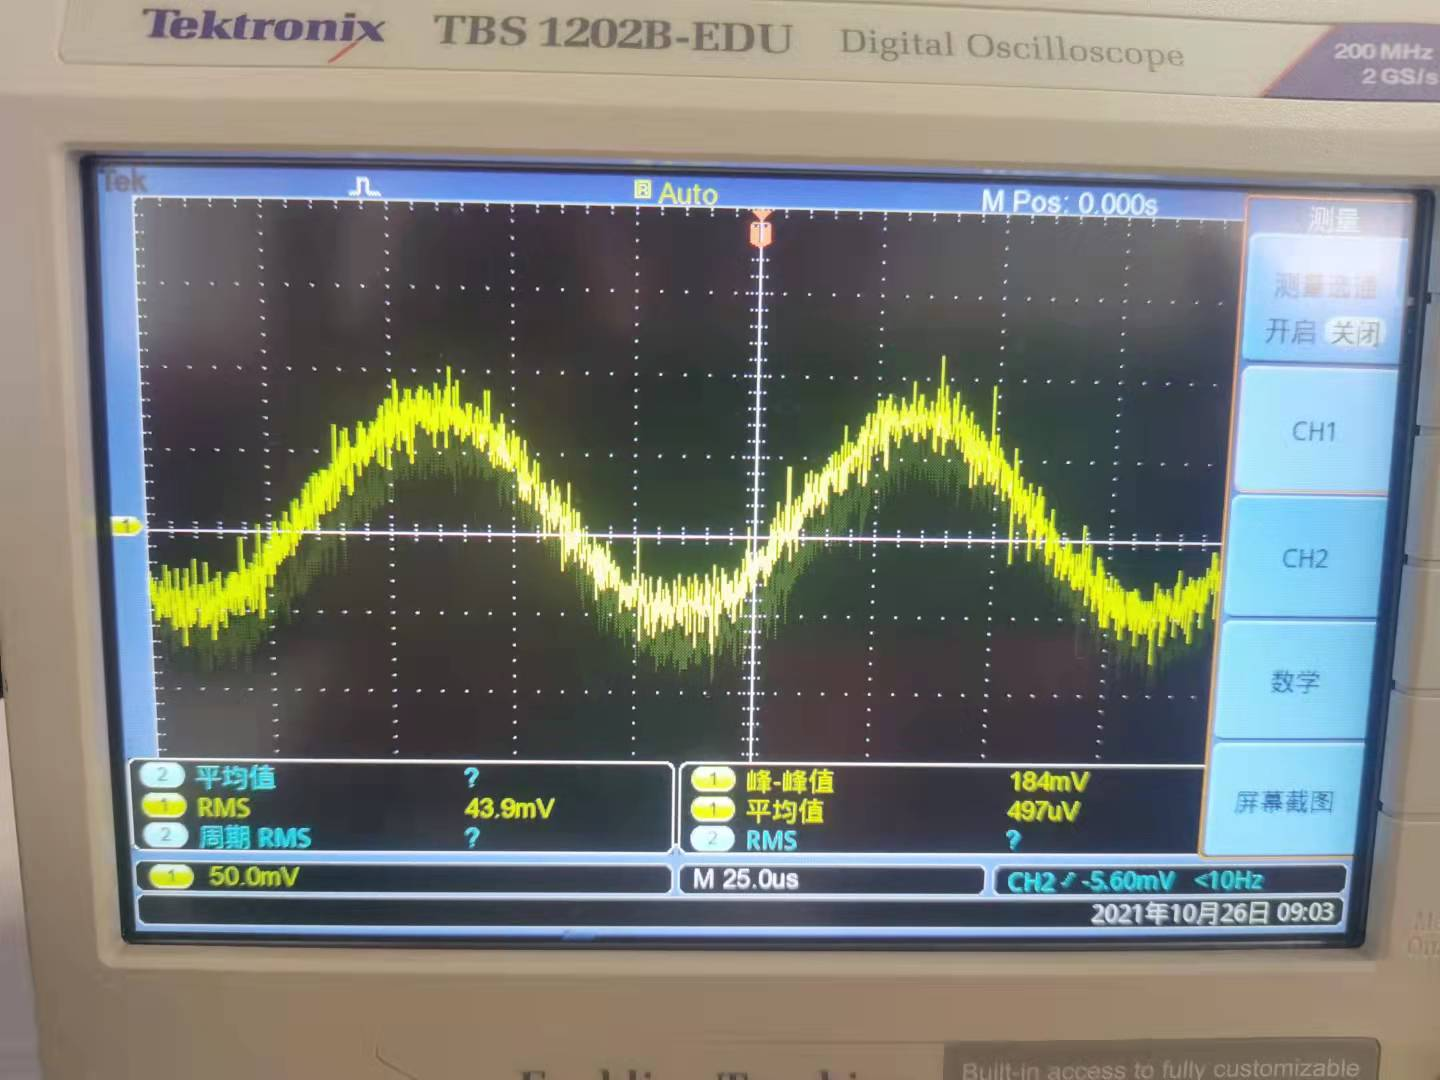
\includegraphics[width=0.60\textwidth]{2-4.jpg}
\end{figure}

计算放大倍数:
\begin{align}
        A_u = \frac{184m}{10\sqrt{2}m} \approx 13.0     
\end{align}

可以看出在串联$100 \Omega$后电路引入了交流负反馈,使得放大倍数减小。


\subsubsection*{(5)将$R_1$更换为 5kΩ电阻,测量静态工作点、输出波形及电压放大倍数等
参数}

将$R_1$改为$5k \Omega$,测量静态工作点如下表:

\begin{table}[H]
    \centering
    \caption{\label{表5}\textbf{更换$R_1$后静态工作点测量}}
    \begin{tabular}{ccc}
    \toprule
            $U_E/V$ & $U_B/V$ &  $U_C/V$\\
    \midrule
            6.79 & 7.43 & 8.64 \\            
    \bottomrule
    \end{tabular}
\end{table}

输入电压为$5mVrms$, 频率为$10kHz$,测量输出波形:

\begin{figure}[htbp]
        \centering
        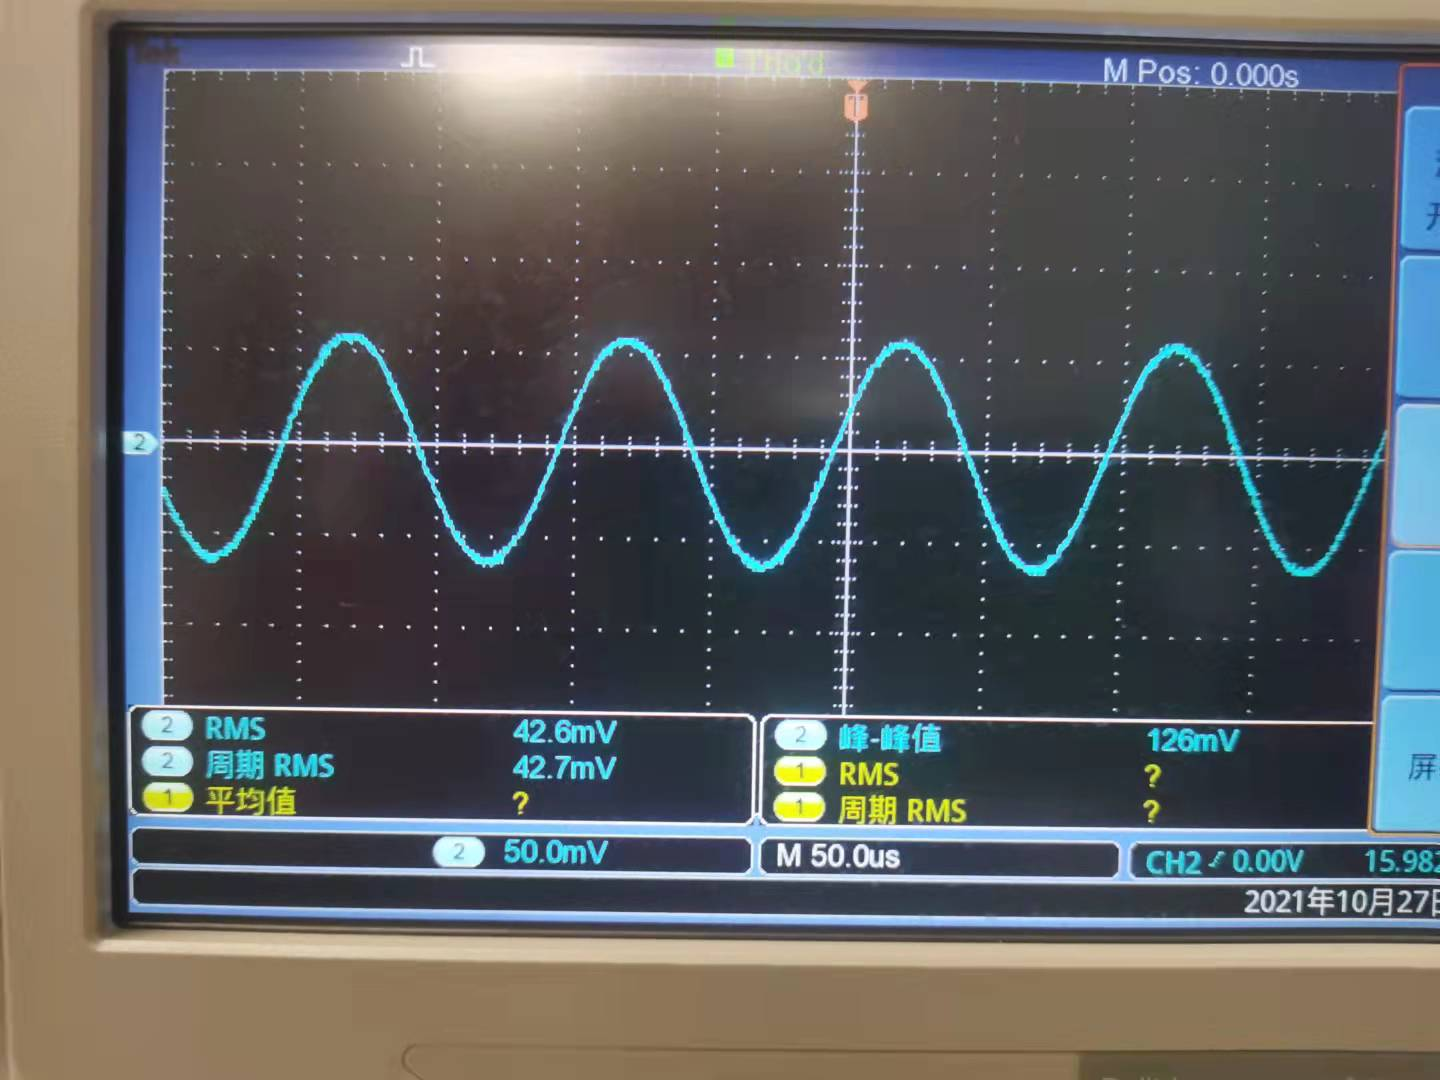
\includegraphics[width=0.60\textwidth]{2-5.jpg}
\end{figure}

由此可以计算出放大倍数:
\begin{align}
        A_u = \frac{U_o}{U_i} = \frac{126m}{10\sqrt{2}m} \approx 8.91 
\end{align}

可以看出电路参数改变,输出电压的值也会改变。

% \
% $Vi=[-7.80, 8.00]   V_o = [-7.80, 6.80] 
% Vi = [-5.2, 5.6]   Vo = [-5.0, 5.60]$

\subsection*{3.用LTspice软件仿真图2所示电路。}

仿真结果如下:
\begin{figure}[htbp]
        \centering
        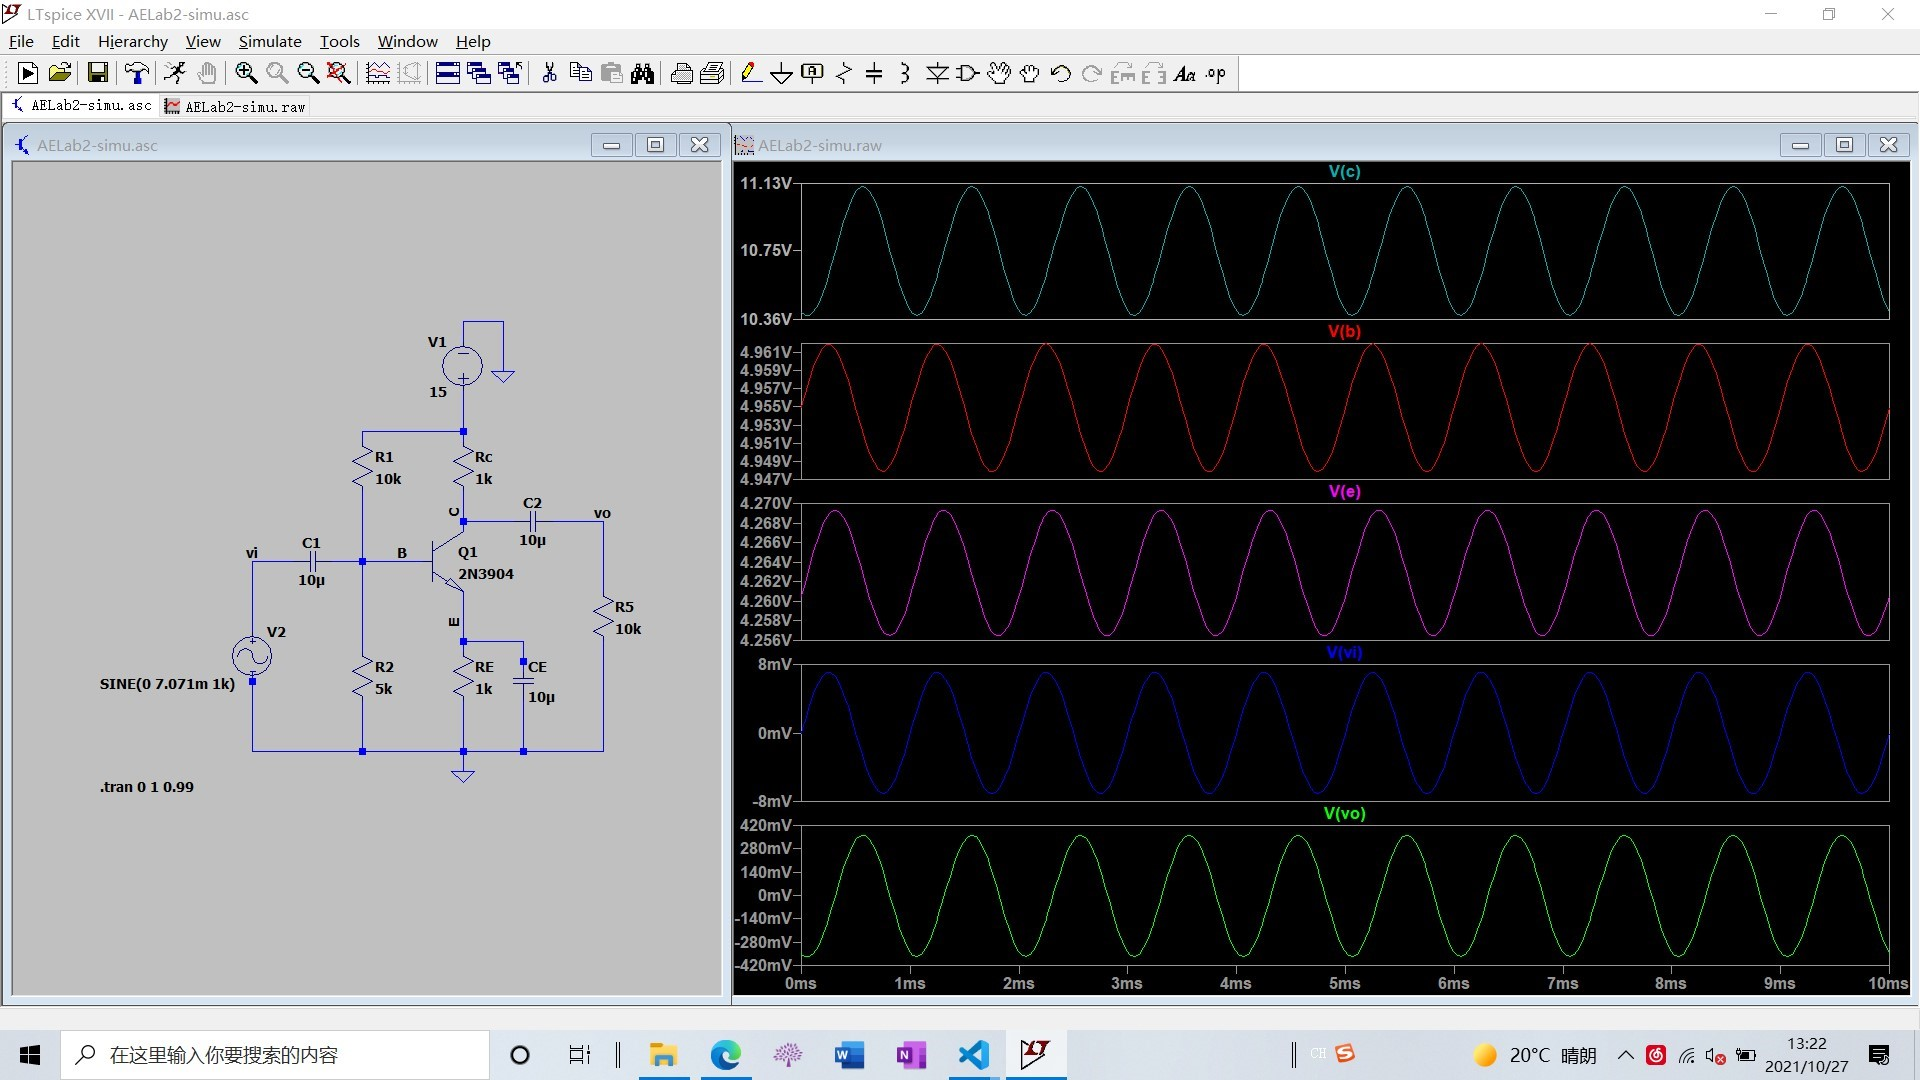
\includegraphics[width=1.0\textwidth]{2-3-1kHz仿真.jpg}
\end{figure}

仿真结果与实验测量结果相近。

\end{document}